\chapter{Irrégularités du bois}

\begin{abstract}
Le bois est un matériau naturel, donc variable par définition. Il présente donc parfois certaines  \og irrégularités  \fg. On rencontre les termes  \og défauts \fg ou  \og anomalies  \fg pour les désigner. Le terme irrégularité est probablement plus approprié puisqu'un défaut ou une anomalie pour un usage donné peut être un avantage pour une autre application. Nous verrons ci-dessous les irrégularités du bois les plus fréquentes.
\end{abstract}

\minitoc

\section{Fil croisé et pente du fil (\textit{Cross-grain and slope of grain})}

Le fil croisé est un terme général désignant la déviation du fil du bois (axe longitudinal des fibres ou trachéides) par rapport à l'axe longitudinal d'un sciage. L'angle formé par l'axe longitudinal des fibres ou trachéides et l'axe longitudinal d'un sciage est appelé pente du fil.\\

Tel qu'illustré à la Figure~\ref{fig:fil}, la pente du fil peut être due à plusieurs causes, entre autres le délignage inapproprié des sciages, le sciage parallèle à l'axe de la bille et le fil spiralé. Le sciage de billes courbes et la présence de nœuds sont également des causes de fil croisé. 

\begin{figure}[h]
	\centering
	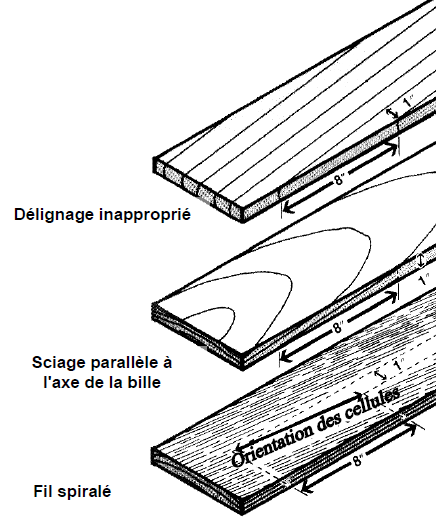
\includegraphics[scale=0.7]{img/ch9_fil}
	\caption{Quelques causes de fil croisé (ou pente du fil) (adapté de \cite{bowyer2007forest})}
	\label{fig:fil}
\end{figure}

\section{Fil spiralé (\textit{Spiral grain})}

Le fil spiralé est dû à l'orientation hélicoïdale des fibres ou des trachéides dans la tige (Figure~\ref{fig:contrefil}a). Cette irrégularité est partiellement héréditaire mais peut être favorisée par la charge en torsion sur la tige induite par l'effet du vent dans la cime, en particulier si cette dernière est non symétrique. Le fil spiralé est surtout observable dans les poteaux et en cause la torsion. Il est souvent confondu avec le fil croisé dans le bois de sciage produit dans des tiges présentant du fil spiralé.

\section{Contrefil (\textit{Interlocked grain})}

Le contrefil résulte de la production de fil spiralé dans une direction pendant quelques années, puis dans l'autre direction et ainsi de suite de façon cyclique (Figure~\ref{fig:contrefil}b et c). Cet effet est héréditaire et se produit surtout chez les bois tropicaux. Il est toutefois présent chez l'orme, ce qui rend ce bois difficile à fendre.

\begin{figure}[h]
	\centering
	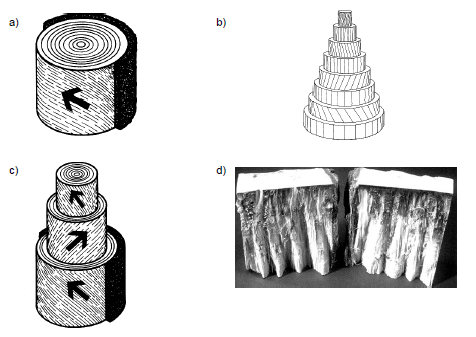
\includegraphics[scale=1]{img/ch9_contrefil}
	\caption{Fil spiralé (a) et contre-fil (b, c, d) (adapté de \cite{bowyer2007forest} et \cite{hoadley1990identifying})}
	\label{fig:contrefil}
\end{figure}

\section{Nœuds (\textit{Knots})}

Les nœuds sont déterminants au niveau des propriétés physico-mécaniques et de la valeur des sciages. En particulier, on classe les sciages visuellement en fonction de l'adhérence, la dimension et la position des nœuds dans la pièce. Tel qu'illustré à la Figure~\ref{fig:adherents}, les nœuds adhérents sont issus des branches vivantes dont le cambium est lié à celui de la tige. Un fois que la branche meurt, le cambium de la tige n'est plus lié à celui de la branche mais le bois produit par le cambium de la tige va la recouvrir graduellement au fil des ans. La branche morte incluse dans la tige formera éventuellement un nœud non adhérent (Figure~\ref{fig:adherents_photos}) si un sciage est produit à cet endroit.

\begin{figure}[h]
	\centering
	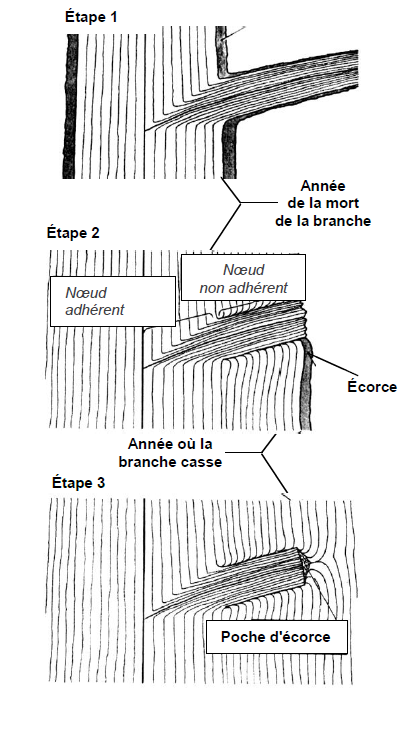
\includegraphics[scale=0.6]{img/ch9_adherents}
	\caption{Formation des nœuds adhérents et non adhérents (adapté de \cite{hoadley1990identifying})}
	\label{fig:adherents}
\end{figure}


\begin{figure}[h]
	\centering
	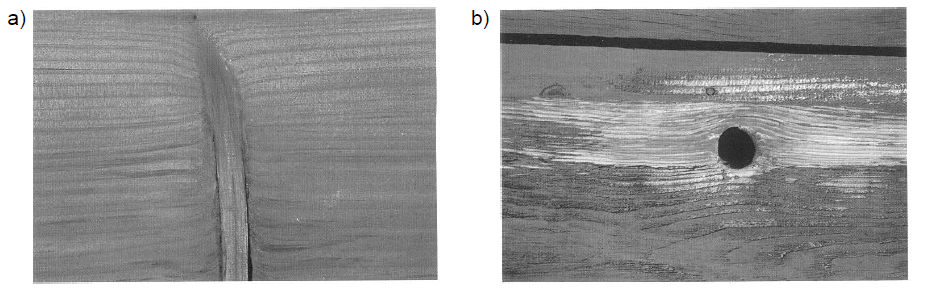
\includegraphics[scale=0.55]{img/ch9_adherents_photos}
	\caption{Nœuds adhérents et non adhérents (adapté de \cite{hoadley1990identifying})}
	\label{fig:adherents_photos}
\end{figure}

\section{Bois de réaction}

Le terme bois de réaction est utilisé pour désigner le bois produit sous l'effet d'une contrainte mécanique. Ce type de bois se retrouve habituellement dans les branches et souvent dans des tiges courbées et/ou croissant dans de fortes pentes. Il a une structure et des propriétés différentes que celles du bois dit  \og normal  \fg. En particulier, la moelle des tiges ou des branches est généralement excentrée et le retrait longitudinal de ce bois est beaucoup plus fort que celui du bois normal. Chez les résineux, le bois de réaction est produit sous l'effet d'une contrainte de compression. On l'appelle donc bois de compression. Comme c'est l'inverse chez les feuillus, on l'appelle bois de tension.

\subsection{Bois de compression}\label{compression}

On retrouve le bois de compression dans la partie inférieure des tiges inclinées et des branches des résineux (Figure~\ref{fig:compression}). La moelle est excentrée, le bois final des cernes annuels étant plus large du côté de la tige en compression. Le bois de compression est plus \og rouge \fg que le bois normal à cause de la plus grande proportion de bois final.\\

Les trachéides du bois de compression en coupe transversale sont circulaires plutôt qu'angulaires comme c'est le cas pour le bois normal (Figure~\ref{fig:compression_micro}). La paroi secondaire des trachéides du bois de compression est environ deux fois plus épaisse que pour le bois normal. En plan tangentiel et radial, on observe souvent des fentes ayant l'apparence \og d'épaississements spiralés \fg dans la paroi S\sub{2} du bois de compression. L'angle des microfibrilles de la paroi S\sub{2} est d'environ 45\textdegree, beaucoup plus que dans la paroi S\sub{2} du bois normal (10 à 30\textdegree). Ceci résulte en un retrait longitudinal environ 10 fois plus grand que pour le bois mature normal. Les trachéides du bois de compression sont 10 à 40\% plus courtes que celles du bois mature. La masse volumique du bois de compression est de 10 à 20\% plus grande que celle du bois mature.

\begin{figure}[h]
	\centering
	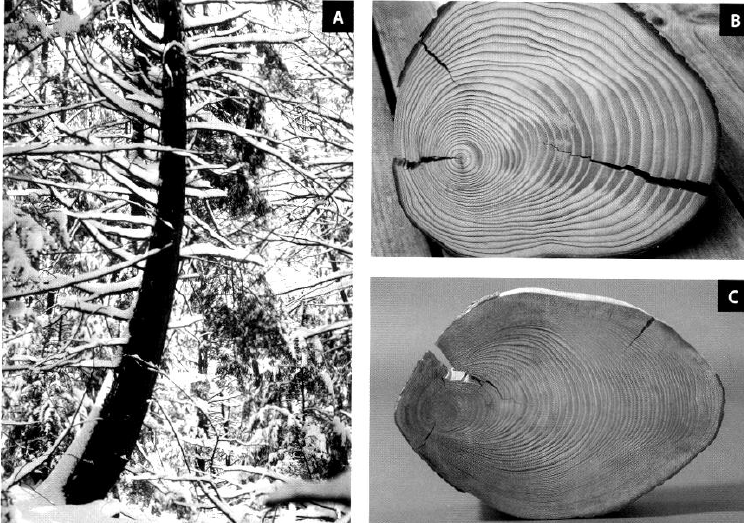
\includegraphics[scale=0.55]{img/ch9_compression}
	\caption{Bois de compression chez les résineux. a) tige courbe contenant typiquement du bois de compression, b) bois de compression chez la pruche, c) bois de compression chez l'épinette (adapté de \cite{hoadley1990identifying})}
	\label{fig:compression}
\end{figure}

\begin{figure}[h]
	\centering
	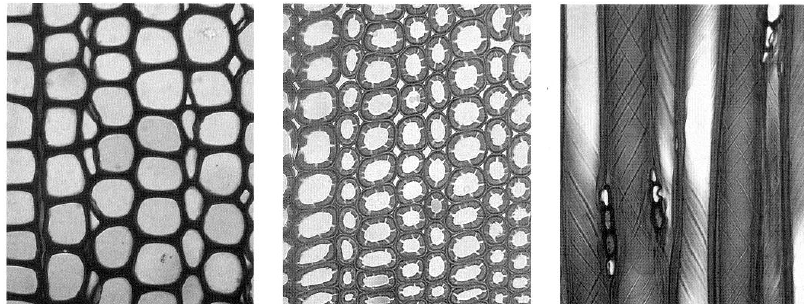
\includegraphics[scale=0.7]{img/ch9_compression_micro}
	\caption{Bois normal (à gauche), bois de compression (au centre et à droite) chez le pin blanc (d'après \cite{hoadley1990identifying})}
	\label{fig:compression_micro}
\end{figure}

\subsection{Bois de tension}

Le bois de tension se retrouve dans la partie supérieure des tiges inclinées et des branches des feuillus, c'est-à-dire dans le bois produit sous l'effet d'une contrainte de tension. La moelle peut être excentrée ou non (Figure~\ref{fig:tension}). Le retrait longitudinal du bois de tension est de un à cinq fois plus grand que celui du bois mature, ce qui en fait un bois ayant tendance à gauchir fortement suite au séchage. Ce bois est difficile à usiner, en particulier de manière à obtenir une surface de belle qualité. Les fibres ont tendance à se relever suite au passage de la raboteuse pour donner une surface peluchée. Au niveau microscopique, les fibres développent une couche interne  \og gélatineuse \fg épaisse et \textbf{non lignifiée} (Figure~\ref{fig:tension_micro}). La présence de bois de tension est particulièrement fréquente chez le bois de peuplier faux-tremble. 

\begin{figure}[h]
	\centering
	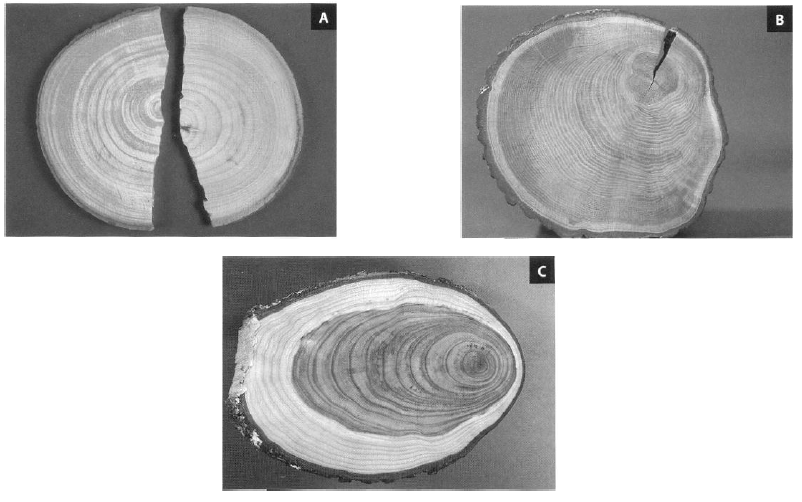
\includegraphics[scale=0.55]{img/ch9_tension}
	\caption{Bois de tension chez les feuillus. a) apparence du bois de tension sans moelle excentrée, b) et c) bois de tension avec moelle excentrée (d'après \cite{hoadley1990identifying})}
	\label{fig:tension}
\end{figure}

\begin{figure}[h]
	\centering
	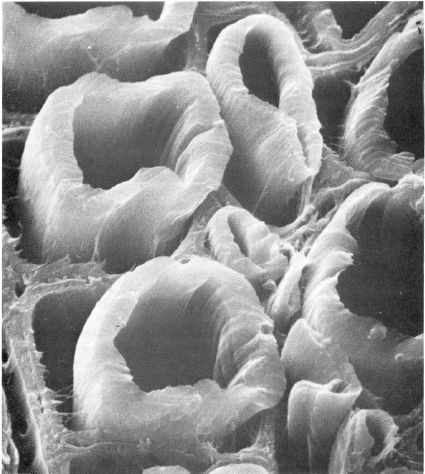
\includegraphics[scale=0.55]{img/ch9_tension_micro}
	\caption{Couche gélatineuse dans les fibres du bois de tension chez le peuplier (d'après \cite{panshin1980textbook})}
	\label{fig:tension_micro}
\end{figure}

\section{Contraintes de croissance (\textit{Growth stresses})}

Le dépôt et la polymérisation de la lignine dans la paroi secondaire des cellules après division à partir du cambium impliquent un gonflement des parois et une diminution de la longueur des cellules (fibres ou trachéides). Cet effet est plus important chez les feuillus que chez les résineux et est particulièrement bien connu chez les eucalyptus. Les contraintes de croissance peuvent causer des fentes importantes dans les billes (Figure~\ref{fig:contraintes}).

\begin{figure}[h]
	\centering
	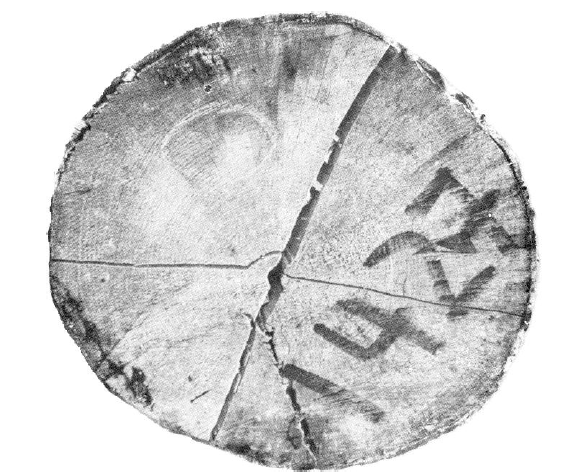
\includegraphics[scale=0.5]{img/ch9_contraintes}
	\caption{Fentes dues aux contraintes de croissance (d'après \cite{panshin1980textbook})}
	\label{fig:contraintes}
\end{figure}

\section{Roulures (\textit{Ring shakes})}

Les roulures sont des séparations du bois à l'interface bois initial -- bois final (Figure~\ref{fig:shake}). Leur cause n'est pas connue précisément mais l'effet du gel, l'action du vent sur les tiges ou la présence de canaux résinifères traumatiques sont souvent mentionnés comme causes probables. Le sapin baumier, la pruche de l'Est et les chênes présentent fréquemment des roulures.

\begin{figure}[h]
	\centering
	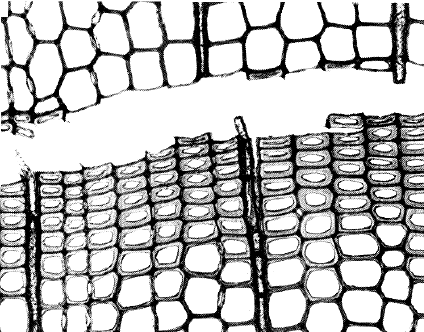
\includegraphics[scale=0.55]{img/ch9_shake}
	\caption{Roulure chez la pruche (d'après \cite{panshin1980textbook})}
	\label{fig:shake}
\end{figure}

\section{Poches de résine (\textit{Pitch pockets})}

Les poches de résine sont surtout présentes chez les espèces possédant normalement des canaux résinifères telles que les épinettes, les mélèzes, les pins et le sapin de Douglas. Elles sont de forme lenticulaire et sont généralement situées à l'intérieur des cernes annuels (Figure~\ref{fig:poches}).

\begin{figure}[h]
	\centering
	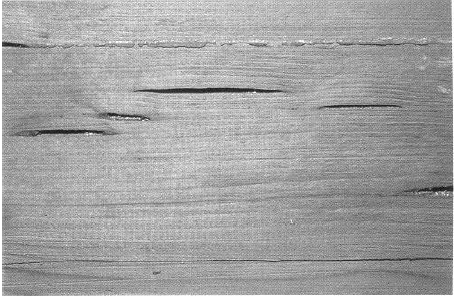
\includegraphics[scale=0.7]{img/ch9_poches}
	\caption{Poches de résine chez l'épinette (d'après \cite{hoadley1990identifying})}
	\label{fig:poches}
\end{figure}

\section{Autres irrégularités}

D'autres irrégularités de la structure du bois peuvent en augmenter la valeur, en particulier pour la fabrication de meubles haut de gamme. L'érable à sucre présente deux irrégularités importantes. L'\og érable ondulé  \fg (\textit{tiger maple}) est dû à l'ondulation du fil du bois. Une fois raboté et vernis, ce bois présente des ondulations très esthétiques. On l'utilise souvent pour la fabrication des violons. L'  \og érable piqué  \fg (\textit{bird's-eye maple}) est une autre irrégularité recherchée pour l'ébénisterie. Des renflements du cambium vers l'intérieur de la tige causent ce dessin typique du bois.





%Références
%
%
%
%Haygreen, J.G.; Bowyer, J.L. 1989. Forest Products and Wood Science : An Introduction. Second Edition. Iowa State University Press, Ames. 500 p. 
%
%
%
%Hoadley, R.B. 1990. Identifying Wood. Accurate results with simple tools. The Taunton Press. Newtown, Connecticut, USA. 223 p. 
%
%
%
%Hoadley, R.B. 2000. Understanding Wood. A craftsman's guide to wood technology. The Taunton Press. Newtown, Connecticut, USA. 280 p. 
%
%
%
%Panshin, A.J.; de Zeeuw, C. 1980. Textbook of wood technology. Fourth edition. McGraw-Hill Book Co. New York. 722 p.